\subsection{Pourquoi décomposer la table ?}
\paragraph{}{Il y a au début une unique table contenant une vingtaine d'attributs. Pour illustrer la redondance et les dépendances fonctionnelles, cet exemple de \textit{tuples} ne sera centré que sur quelques attributs pour des raisons de lisibilité. LA figure \ref{bigtableex} présente un aperçu de notre \textit{big table}.}

\begin{figure}
\label{bigtableex}
    {
	\centering
    \begin{tabular}{|l|l|l|l|l|l|l|l|}
        \hline idArt & titreArt & idJrnal & typeJrnal & idCont & nomCont & nomPers & nomMetier \\ 
        \hline 1 & Les pieuvres & 1 & Hebdo & 1 & Photo & Bertrand & Photographe \\ 
        \hline 1 & Les pieuvres & 1 & Hebdo & 2 &Texte & Nadine & Redacteur \\ 
        \hline 2 & Manger du sel & 1 & Hebdo & 3 & Schéma & Yves & Infographie \\ 
        \hline 2 & Manger du sel & 1 & Hebdo & 4 & Texte & Nadine & Redacteur \\ 
        \hline 3 & Critique film & 1 & Hebdo & 5 & Texte & Manon & Critique \\ 
        \hline 4 & Des poissons & 3 & HS & 6 & Texte & Nadine & Redacteur \\ 
        \hline 2 & Manger du sel & 3 & HS & 1 & Schéma & Yves & Infographie \\ 
        \hline 2 & Manger du sel & 3 & HS & 2 & Texte & Nadine & Redacteur \\ 
        \hline 
    \end{tabular}
    }
\caption{Exemple de \textit{tuples} dans la \textit{big table} (vue partielle)}
\end{figure} 

\paragraph{}{On remarque qu'il a une répétition des données relatives au journal ou au contenu : un contenu a toujours les mêmes ID, nom et auteur associé. Les journaux d'un même ID ont leur type en commun, de même pour les IDs d'es articles et leurs titres. Enfin, les personnes ont toujours le même métier. On peut avoir une perte d'information du fait de cette configuration car si l'on supprime par exemple tous les contenus créés par une personne, on perd les données qui lui sont associées, à savoir son nom, son prénom, son numéro, etc.}

\paragraph{}{De ce fait, en prenant en compte tous les attributs nous avons dégagé un ensemble de dépendances fonctionnelles entre ceux-ci.}

\begin{figure}
	\label{sch_df}
	\centering
	\ifx\du\undefined
  \newlength{\du}
\fi
\setlength{\du}{15\unitlength}
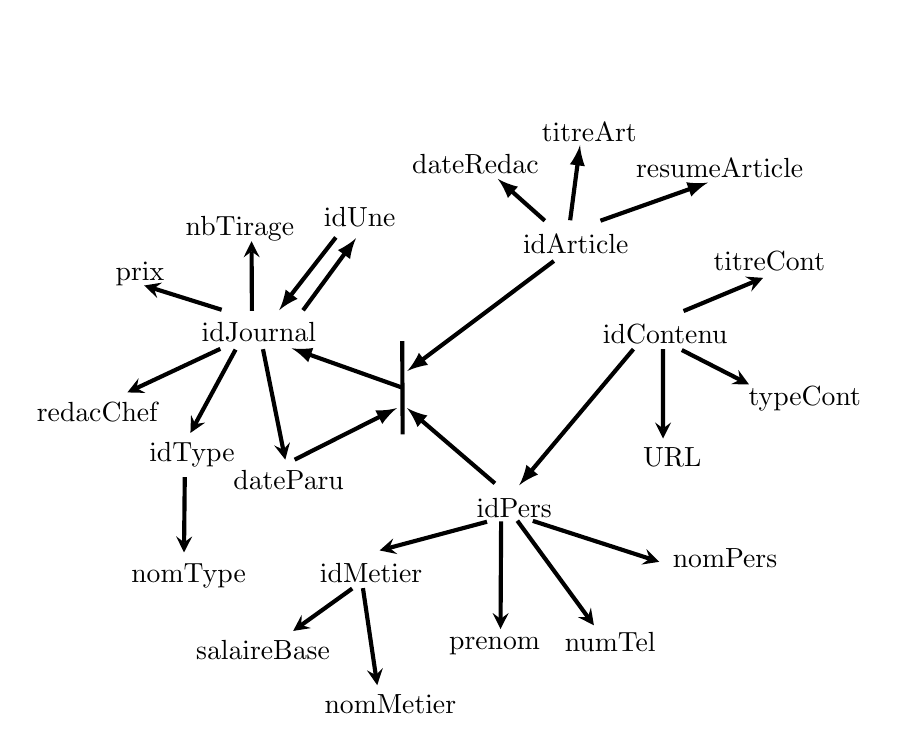
\begin{tikzpicture}[scale=0.9]
\pgftransformxscale{1.000000}
\pgftransformyscale{-1.000000}
\definecolor{dialinecolor}{rgb}{0.000000, 0.000000, 0.000000}
\pgfsetstrokecolor{dialinecolor}
\definecolor{dialinecolor}{rgb}{1.000000, 1.000000, 1.000000}
\pgfsetfillcolor{dialinecolor}
% setfont left to latex
\definecolor{dialinecolor}{rgb}{0.000000, 0.000000, 0.000000}
\pgfsetstrokecolor{dialinecolor}
\node[anchor=west] at (29.900000\du,17.850000\du){idPers};
% setfont left to latex
\definecolor{dialinecolor}{rgb}{0.000000, 0.000000, 0.000000}
\pgfsetstrokecolor{dialinecolor}
\node[anchor=west] at (35.150000\du,19.200000\du){nomPers};
% setfont left to latex
\definecolor{dialinecolor}{rgb}{0.000000, 0.000000, 0.000000}
\pgfsetstrokecolor{dialinecolor}
\node[anchor=west] at (29.163689\du,21.565612\du){prenom};
% setfont left to latex
\definecolor{dialinecolor}{rgb}{0.000000, 0.000000, 0.000000}
\pgfsetstrokecolor{dialinecolor}
\node[anchor=west] at (32.259087\du,21.436290\du){numTel};
% setfont left to latex
\definecolor{dialinecolor}{rgb}{0.000000, 0.000000, 0.000000}
\pgfsetstrokecolor{dialinecolor}
\node[anchor=west] at (25.706125\du,19.600000\du){idMetier};
% setfont left to latex
\definecolor{dialinecolor}{rgb}{0.000000, 0.000000, 0.000000}
\pgfsetstrokecolor{dialinecolor}
\node[anchor=west] at (30.500000\du,21.600000\du){};
% setfont left to latex
\definecolor{dialinecolor}{rgb}{0.000000, 0.000000, 0.000000}
\pgfsetstrokecolor{dialinecolor}
\node[anchor=west] at (25.828978\du,23.102844\du){nomMetier};
\pgfsetlinewidth{0.100000\du}
\pgfsetdash{}{0pt}
\pgfsetdash{}{0pt}
\pgfsetbuttcap
{
\definecolor{dialinecolor}{rgb}{0.000000, 0.000000, 0.000000}
\pgfsetfillcolor{dialinecolor}
% was here!!!
\pgfsetarrowsend{stealth}
\definecolor{dialinecolor}{rgb}{0.000000, 0.000000, 0.000000}
\pgfsetstrokecolor{dialinecolor}
\draw (30.437875\du,18.227601\du)--(27.564463\du,18.995588\du);
}
\pgfsetlinewidth{0.100000\du}
\pgfsetdash{}{0pt}
\pgfsetdash{}{0pt}
\pgfsetbuttcap
{
\definecolor{dialinecolor}{rgb}{0.000000, 0.000000, 0.000000}
\pgfsetfillcolor{dialinecolor}
% was here!!!
\pgfsetarrowsend{stealth}
\definecolor{dialinecolor}{rgb}{0.000000, 0.000000, 0.000000}
\pgfsetstrokecolor{dialinecolor}
\draw (30.816138\du,18.216138\du)--(30.800000\du,21.100000\du);
}
\pgfsetlinewidth{0.100000\du}
\pgfsetdash{}{0pt}
\pgfsetdash{}{0pt}
\pgfsetbuttcap
{
\definecolor{dialinecolor}{rgb}{0.000000, 0.000000, 0.000000}
\pgfsetfillcolor{dialinecolor}
% was here!!!
\pgfsetarrowsend{stealth}
\definecolor{dialinecolor}{rgb}{0.000000, 0.000000, 0.000000}
\pgfsetstrokecolor{dialinecolor}
\draw (31.250000\du,18.200000\du)--(33.300000\du,21.000000\du);
}
\pgfsetlinewidth{0.100000\du}
\pgfsetdash{}{0pt}
\pgfsetdash{}{0pt}
\pgfsetbuttcap
{
\definecolor{dialinecolor}{rgb}{0.000000, 0.000000, 0.000000}
\pgfsetfillcolor{dialinecolor}
% was here!!!
\pgfsetarrowsend{stealth}
\definecolor{dialinecolor}{rgb}{0.000000, 0.000000, 0.000000}
\pgfsetstrokecolor{dialinecolor}
\draw (31.664363\du,18.204676\du)--(35.050000\du,19.300000\du);
}
\pgfsetlinewidth{0.100000\du}
\pgfsetdash{}{0pt}
\pgfsetdash{}{0pt}
\pgfsetbuttcap
{
\definecolor{dialinecolor}{rgb}{0.000000, 0.000000, 0.000000}
\pgfsetfillcolor{dialinecolor}
% was here!!!
\pgfsetarrowsend{stealth}
\definecolor{dialinecolor}{rgb}{0.000000, 0.000000, 0.000000}
\pgfsetstrokecolor{dialinecolor}
\draw (27.117425\du,20.004288\du)--(27.500000\du,22.600000\du);
}
% setfont left to latex
\definecolor{dialinecolor}{rgb}{0.000000, 0.000000, 0.000000}
\pgfsetstrokecolor{dialinecolor}
\node[anchor=west] at (22.500000\du,13.150000\du){idJournal};
% setfont left to latex
\definecolor{dialinecolor}{rgb}{0.000000, 0.000000, 0.000000}
\pgfsetstrokecolor{dialinecolor}
\node[anchor=west] at (18.088100\du,15.300000\du){redacChef};
% setfont left to latex
\definecolor{dialinecolor}{rgb}{0.000000, 0.000000, 0.000000}
\pgfsetstrokecolor{dialinecolor}
\node[anchor=west] at (23.348812\du,17.097434\du){dateParu};
% setfont left to latex
\definecolor{dialinecolor}{rgb}{0.000000, 0.000000, 0.000000}
\pgfsetstrokecolor{dialinecolor}
\node[anchor=west] at (21.096837\du,16.438537\du){idType};
% setfont left to latex
\definecolor{dialinecolor}{rgb}{0.000000, 0.000000, 0.000000}
\pgfsetstrokecolor{dialinecolor}
\node[anchor=west] at (20.198549\du,11.592687\du){prix};
% setfont left to latex
\definecolor{dialinecolor}{rgb}{0.000000, 0.000000, 0.000000}
\pgfsetstrokecolor{dialinecolor}
\node[anchor=west] at (22.069695\du,10.376113\du){nbTirage};
\pgfsetlinewidth{0.100000\du}
\pgfsetdash{}{0pt}
\pgfsetdash{}{0pt}
\pgfsetbuttcap
{
\definecolor{dialinecolor}{rgb}{0.000000, 0.000000, 0.000000}
\pgfsetfillcolor{dialinecolor}
% was here!!!
\pgfsetarrowsend{stealth}
\definecolor{dialinecolor}{rgb}{0.000000, 0.000000, 0.000000}
\pgfsetstrokecolor{dialinecolor}
\draw (23.300000\du,13.600000\du)--(20.812463\du,14.765925\du);
}
\pgfsetlinewidth{0.100000\du}
\pgfsetdash{}{0pt}
\pgfsetdash{}{0pt}
\pgfsetbuttcap
{
\definecolor{dialinecolor}{rgb}{0.000000, 0.000000, 0.000000}
\pgfsetfillcolor{dialinecolor}
% was here!!!
\pgfsetarrowsend{stealth}
\definecolor{dialinecolor}{rgb}{0.000000, 0.000000, 0.000000}
\pgfsetstrokecolor{dialinecolor}
\draw (23.708460\du,13.619674\du)--(22.500000\du,15.850000\du);
}
\pgfsetlinewidth{0.100000\du}
\pgfsetdash{}{0pt}
\pgfsetdash{}{0pt}
\pgfsetbuttcap
{
\definecolor{dialinecolor}{rgb}{0.000000, 0.000000, 0.000000}
\pgfsetfillcolor{dialinecolor}
% was here!!!
\pgfsetarrowsend{stealth}
\definecolor{dialinecolor}{rgb}{0.000000, 0.000000, 0.000000}
\pgfsetstrokecolor{dialinecolor}
\draw (24.442061\du,13.608212\du)--(25.038323\du,16.565538\du);
}
\pgfsetlinewidth{0.100000\du}
\pgfsetdash{}{0pt}
\pgfsetdash{}{0pt}
\pgfsetbuttcap
{
\definecolor{dialinecolor}{rgb}{0.000000, 0.000000, 0.000000}
\pgfsetfillcolor{dialinecolor}
% was here!!!
\pgfsetarrowsend{stealth}
\definecolor{dialinecolor}{rgb}{0.000000, 0.000000, 0.000000}
\pgfsetstrokecolor{dialinecolor}
\draw (22.348439\du,17.035500\du)--(22.327700\du,19.050000\du);
}
\pgfsetlinewidth{0.100000\du}
\pgfsetdash{}{0pt}
\pgfsetdash{}{0pt}
\pgfsetbuttcap
{
\definecolor{dialinecolor}{rgb}{0.000000, 0.000000, 0.000000}
\pgfsetfillcolor{dialinecolor}
% was here!!!
\pgfsetarrowsend{stealth}
\definecolor{dialinecolor}{rgb}{0.000000, 0.000000, 0.000000}
\pgfsetstrokecolor{dialinecolor}
\draw (23.335575\du,12.554150\du)--(21.263275\du,11.904150\du);
}
\pgfsetlinewidth{0.100000\du}
\pgfsetdash{}{0pt}
\pgfsetdash{}{0pt}
\pgfsetbuttcap
{
\definecolor{dialinecolor}{rgb}{0.000000, 0.000000, 0.000000}
\pgfsetfillcolor{dialinecolor}
% was here!!!
\pgfsetarrowsend{stealth}
\definecolor{dialinecolor}{rgb}{0.000000, 0.000000, 0.000000}
\pgfsetstrokecolor{dialinecolor}
\draw (24.145850\du,12.581225\du)--(24.135338\du,10.719661\du);
}
% setfont left to latex
\definecolor{dialinecolor}{rgb}{0.000000, 0.000000, 0.000000}
\pgfsetstrokecolor{dialinecolor}
\node[anchor=west] at (31.100000\du,10.800000\du){idArticle};
% setfont left to latex
\definecolor{dialinecolor}{rgb}{0.000000, 0.000000, 0.000000}
\pgfsetstrokecolor{dialinecolor}
\node[anchor=west] at (28.400000\du,5.250000\du){};
% setfont left to latex
\definecolor{dialinecolor}{rgb}{0.000000, 0.000000, 0.000000}
\pgfsetstrokecolor{dialinecolor}
\node[anchor=west] at (31.605687\du,7.800000\du){titreArt};
% setfont left to latex
\definecolor{dialinecolor}{rgb}{0.000000, 0.000000, 0.000000}
\pgfsetstrokecolor{dialinecolor}
\node[anchor=west] at (28.131821\du,8.650000\du){dateRedac};
% setfont left to latex
\definecolor{dialinecolor}{rgb}{0.000000, 0.000000, 0.000000}
\pgfsetstrokecolor{dialinecolor}
\node[anchor=west] at (33.239777\du,13.200000\du){idContenu};
% setfont left to latex
\definecolor{dialinecolor}{rgb}{0.000000, 0.000000, 0.000000}
\pgfsetstrokecolor{dialinecolor}
\node[anchor=west] at (36.200000\du,11.250000\du){titreCont};
% setfont left to latex
\definecolor{dialinecolor}{rgb}{0.000000, 0.000000, 0.000000}
\pgfsetstrokecolor{dialinecolor}
\node[anchor=west] at (34.313643\du,16.500000\du){URL};
% setfont left to latex
\definecolor{dialinecolor}{rgb}{0.000000, 0.000000, 0.000000}
\pgfsetstrokecolor{dialinecolor}
\node[anchor=west] at (37.139777\du,14.936933\du){typeCont};
\pgfsetlinewidth{0.100000\du}
\pgfsetdash{}{0pt}
\pgfsetdash{}{0pt}
\pgfsetbuttcap
{
\definecolor{dialinecolor}{rgb}{0.000000, 0.000000, 0.000000}
\pgfsetfillcolor{dialinecolor}
% was here!!!
\pgfsetarrowsend{stealth}
\definecolor{dialinecolor}{rgb}{0.000000, 0.000000, 0.000000}
\pgfsetstrokecolor{dialinecolor}
\draw (35.699164\du,12.588049\du)--(37.827700\du,11.700000\du);
}
\pgfsetlinewidth{0.100000\du}
\pgfsetdash{}{0pt}
\pgfsetdash{}{0pt}
\pgfsetbuttcap
{
\definecolor{dialinecolor}{rgb}{0.000000, 0.000000, 0.000000}
\pgfsetfillcolor{dialinecolor}
% was here!!!
\pgfsetarrowsend{stealth}
\definecolor{dialinecolor}{rgb}{0.000000, 0.000000, 0.000000}
\pgfsetstrokecolor{dialinecolor}
\draw (35.148964\du,13.608212\du)--(35.150000\du,16.000000\du);
}
\pgfsetlinewidth{0.100000\du}
\pgfsetdash{}{0pt}
\pgfsetdash{}{0pt}
\pgfsetbuttcap
{
\definecolor{dialinecolor}{rgb}{0.000000, 0.000000, 0.000000}
\pgfsetfillcolor{dialinecolor}
% was here!!!
\pgfsetarrowsend{stealth}
\definecolor{dialinecolor}{rgb}{0.000000, 0.000000, 0.000000}
\pgfsetstrokecolor{dialinecolor}
\draw (35.653314\du,13.631137\du)--(37.450000\du,14.550000\du);
}
% setfont left to latex
\definecolor{dialinecolor}{rgb}{0.000000, 0.000000, 0.000000}
\pgfsetstrokecolor{dialinecolor}
\node[anchor=west] at (22.350000\du,21.665911\du){salaireBase};
\pgfsetlinewidth{0.100000\du}
\pgfsetdash{}{0pt}
\pgfsetdash{}{0pt}
\pgfsetbuttcap
{
\definecolor{dialinecolor}{rgb}{0.000000, 0.000000, 0.000000}
\pgfsetfillcolor{dialinecolor}
% was here!!!
\pgfsetarrowsend{stealth}
\definecolor{dialinecolor}{rgb}{0.000000, 0.000000, 0.000000}
\pgfsetstrokecolor{dialinecolor}
\draw (26.830862\du,20.015751\du)--(25.250000\du,21.150000\du);
}
\pgfsetlinewidth{0.100000\du}
\pgfsetdash{}{0pt}
\pgfsetdash{}{0pt}
\pgfsetbuttcap
{
\definecolor{dialinecolor}{rgb}{0.000000, 0.000000, 0.000000}
\pgfsetfillcolor{dialinecolor}
% was here!!!
\pgfsetarrowsend{latex}
\definecolor{dialinecolor}{rgb}{0.000000, 0.000000, 0.000000}
\pgfsetstrokecolor{dialinecolor}
\draw (34.358051\du,13.608212\du)--(31.300000\du,17.250000\du);
}
\pgfsetlinewidth{0.100000\du}
\pgfsetdash{}{0pt}
\pgfsetdash{}{0pt}
\pgfsetbuttcap
{
\definecolor{dialinecolor}{rgb}{0.000000, 0.000000, 0.000000}
\pgfsetfillcolor{dialinecolor}
% was here!!!
\pgfsetarrowsend{latex}
\definecolor{dialinecolor}{rgb}{0.000000, 0.000000, 0.000000}
\pgfsetstrokecolor{dialinecolor}
\draw (30.650000\du,17.200000\du)--(28.298990\du,15.185069\du);
}
\pgfsetlinewidth{0.100000\du}
\pgfsetdash{}{0pt}
\pgfsetdash{}{0pt}
\pgfsetbuttcap
{
\definecolor{dialinecolor}{rgb}{0.000000, 0.000000, 0.000000}
\pgfsetfillcolor{dialinecolor}
% was here!!!
\pgfsetarrowsend{latex}
\definecolor{dialinecolor}{rgb}{0.000000, 0.000000, 0.000000}
\pgfsetstrokecolor{dialinecolor}
\draw (32.227700\du,11.250000\du)--(28.304924\du,14.192800\du);
}
\pgfsetlinewidth{0.100000\du}
\pgfsetdash{}{0pt}
\pgfsetdash{}{0pt}
\pgfsetbuttcap
{
\definecolor{dialinecolor}{rgb}{0.000000, 0.000000, 0.000000}
\pgfsetfillcolor{dialinecolor}
% was here!!!
\definecolor{dialinecolor}{rgb}{0.000000, 0.000000, 0.000000}
\pgfsetstrokecolor{dialinecolor}
\draw (28.169049\du,13.390424\du)--(28.180511\du,15.889250\du);
}
% setfont left to latex
\definecolor{dialinecolor}{rgb}{0.000000, 0.000000, 0.000000}
\pgfsetstrokecolor{dialinecolor}
\node[anchor=west] at (20.614633\du,19.665911\du){nomType};
\pgfsetlinewidth{0.100000\du}
\pgfsetdash{}{0pt}
\pgfsetdash{}{0pt}
\pgfsetbuttcap
{
\definecolor{dialinecolor}{rgb}{0.000000, 0.000000, 0.000000}
\pgfsetfillcolor{dialinecolor}
% was here!!!
\pgfsetarrowsend{latex}
\definecolor{dialinecolor}{rgb}{0.000000, 0.000000, 0.000000}
\pgfsetstrokecolor{dialinecolor}
\draw (25.290499\du,16.565538\du)--(28.025700\du,15.185069\du);
}
\pgfsetlinewidth{0.100000\du}
\pgfsetdash{}{0pt}
\pgfsetdash{}{0pt}
\pgfsetbuttcap
{
\definecolor{dialinecolor}{rgb}{0.000000, 0.000000, 0.000000}
\pgfsetfillcolor{dialinecolor}
% was here!!!
\pgfsetarrowsend{latex}
\definecolor{dialinecolor}{rgb}{0.000000, 0.000000, 0.000000}
\pgfsetstrokecolor{dialinecolor}
\draw (28.174780\du,14.639837\du)--(25.210048\du,13.585287\du);
}
% setfont left to latex
\definecolor{dialinecolor}{rgb}{0.000000, 0.000000, 0.000000}
\pgfsetstrokecolor{dialinecolor}
\node[anchor=west] at (34.127700\du,8.750000\du){resumeArticle};
\pgfsetlinewidth{0.100000\du}
\pgfsetdash{}{0pt}
\pgfsetdash{}{0pt}
\pgfsetbuttcap
{
\definecolor{dialinecolor}{rgb}{0.000000, 0.000000, 0.000000}
\pgfsetfillcolor{dialinecolor}
% was here!!!
\pgfsetarrowsend{latex}
\definecolor{dialinecolor}{rgb}{0.000000, 0.000000, 0.000000}
\pgfsetstrokecolor{dialinecolor}
\draw (31.985313\du,10.169461\du)--(30.727700\du,9.050000\du);
}
\pgfsetlinewidth{0.100000\du}
\pgfsetdash{}{0pt}
\pgfsetdash{}{0pt}
\pgfsetbuttcap
{
\definecolor{dialinecolor}{rgb}{0.000000, 0.000000, 0.000000}
\pgfsetfillcolor{dialinecolor}
% was here!!!
\pgfsetarrowsend{latex}
\definecolor{dialinecolor}{rgb}{0.000000, 0.000000, 0.000000}
\pgfsetstrokecolor{dialinecolor}
\draw (32.663911\du,10.157999\du)--(32.927700\du,8.150000\du);
}
\pgfsetlinewidth{0.100000\du}
\pgfsetdash{}{0pt}
\pgfsetdash{}{0pt}
\pgfsetbuttcap
{
\definecolor{dialinecolor}{rgb}{0.000000, 0.000000, 0.000000}
\pgfsetfillcolor{dialinecolor}
% was here!!!
\pgfsetarrowsend{latex}
\definecolor{dialinecolor}{rgb}{0.000000, 0.000000, 0.000000}
\pgfsetstrokecolor{dialinecolor}
\draw (33.475438\du,10.169461\du)--(36.350000\du,9.150000\du);
}
\pgfsetlinewidth{0.100000\du}
\pgfsetdash{}{0pt}
\pgfsetdash{}{0pt}
\pgfsetbuttcap
{
\definecolor{dialinecolor}{rgb}{0.000000, 0.000000, 0.000000}
\pgfsetfillcolor{dialinecolor}
% was here!!!
\pgfsetarrowsend{latex}
\definecolor{dialinecolor}{rgb}{0.000000, 0.000000, 0.000000}
\pgfsetstrokecolor{dialinecolor}
\draw (26.392361\du,10.616499\du)--(24.875525\du,12.564625\du);
}
% setfont left to latex
\definecolor{dialinecolor}{rgb}{0.000000, 0.000000, 0.000000}
\pgfsetstrokecolor{dialinecolor}
\node[anchor=west] at (25.772362\du,10.080562\du){idUne};
\pgfsetlinewidth{0.100000\du}
\pgfsetdash{}{0pt}
\pgfsetdash{}{0pt}
\pgfsetbuttcap
{
\definecolor{dialinecolor}{rgb}{0.000000, 0.000000, 0.000000}
\pgfsetfillcolor{dialinecolor}
% was here!!!
\pgfsetarrowsend{latex}
\definecolor{dialinecolor}{rgb}{0.000000, 0.000000, 0.000000}
\pgfsetstrokecolor{dialinecolor}
\draw (25.514962\du,12.567137\du)--(26.931099\du,10.639424\du);
}
% setfont left to latex
\definecolor{dialinecolor}{rgb}{0.000000, 0.000000, 0.000000}
\pgfsetstrokecolor{dialinecolor}
\node[anchor=west] at (29.750000\du,21.450000\du){};
\end{tikzpicture}
	\caption{Schéma des dépendances fonctionnelles de la base de données}
\end{figure} 

\paragraph{Dépendances fonctionnelles}{Les dépendances fonctionnelles de la figure \ref{sch_df} peuvent être retranscrites de la manière suivante.
}
\begin{enumerate}
    \item[(1)] idJournal $\rightarrow$ prix, nbTirage, idUne, idType, redacChef, dateParu
    \item[(2)] idType $\rightarrow$ nomType
    \item[(3)] idUne $\rightarrow$ idJournal
    \item[(4)] idArticle $\rightarrow$ dateRedac, titreArt, resumeArt
    \item[(5)] idContenu $\rightarrow$ URL, titreCont, typeCont
    \item[(6)] idPers $\rightarrow$ nomPers, prenom, numTel, idMetier
    \item[(7)] idMetier $\rightarrow$ salaireBase, nomMetier
    \item[(8)] idArticle, idPers, dateParu $\rightarrow$ idJournal
\end{enumerate}

\paragraph{Clés}{
    De ce schéma, on peut en déduire trois clés $\{idJournal, idArticle, idContenu\}$, $\{idUne, idArticle, idContenu\}$ et $\{dateParu, idContenu, idArticle\}$.
}

\subsection{Algorithme de Bernstein}
\paragraph{}{Une fois nos dépendances fonctionnelles établies, nous commençons par appliquer l'algorithme de Bernstein pour décomposer notre grande table. Tout d'abord, nous déterminons sa couverture minimale. Pour cela, on utilise la clé \{idJournal, idArticle, idContenu\}.
}

\paragraph{}{
    Les dépendances (1), (4), (5), (6) et (7) ne sont pas élémentaires, nous avons donc les décomposer. Toutes les relations n'ont qu'un seul attributs à gauche, il n'est donc pas nécessaire de calculer la fermeture de ces attributs. Mais il est cependant nécessaire de le faire pour la dépendance (8) qui a plus d'un attribut en partie gauche.
    }

\paragraph{}{
    Calcul de la fermeture des attributs en partie gauche de la dépendance fonctionnelle (8) :
}
\begin{itemize}
    \item $idArticle+ = \{dateRedac, titreArt, resumeArticle\}$
    \item $idPers+ = \{nomPers, numTel, prenom, idMetier, nomMetier, salaireBase\}$
    \item $dateParu+ = \{\}$
\end{itemize}

\paragraph{}{Comme aucun élément des trois fermetures n'apparaît en partie gauche de la dépendance (8), cette dernière n'a pas besoin d'être modifiée.}
\paragraph{Couverture minimale}{
\begin{enumerate}
    \item[(1.1)] idJournal $\rightarrow$ prix
    \item[(1.2)] idJournal $\rightarrow$ nbTirage
    \item[(1.3)] idJournal $\rightarrow$ idUne
    \item[(1.4)] idJournal $\rightarrow$ idType
    \item[(1.5)] idJournal $\rightarrow$ redacChef
    \item[(1.6)] idJournal $\rightarrow$ dateParu
    \item[(2)] idType $\rightarrow$ nomType
    \item[(3)] idUne $\rightarrow$ idJournal
    \item[(4.1)] idArticle $\rightarrow$ dateRedac
    \item[(4.2)] idArticle $\rightarrow$ titreArt
    \item[(4.3)] idArticle $\rightarrow$ resumeArt
    \item[(5.1)] idContenu $\rightarrow$ URL
    \item[(5.2)] idContenu $\rightarrow$ titreCont
    \item[(5.3)] idContenu $\rightarrow$ typeCont
    \item[(6.1)] idPers $\rightarrow$ nomPers
    \item[(6.2)] idPers $\rightarrow$ prénom
    \item[(6.3)] idPers $\rightarrow$ numTel
    \item[(6.4)] idPers $\rightarrow$ idMetier
    \item[(7.1)] idMetier $\rightarrow$ salaireBase
    \item[(7.2)] idMetier $\rightarrow$ nomMetier
    \item[(8)] idArticle, idPers, dateParu $\rightarrow$ idJournal
\end{enumerate}}

\paragraph{}{
    Nous regroupons maintenant les dépendances ayant même partie gauche comme ci-dessous.
}
\begin{enumerate}
    \item[(1)] $DF_{1} = \{ (1.1), (1.2), (1.3), (1.4), (1.5), (1.6) \}$
    \item[(2)] $DF_{2} = \{ (2) \}$
    \item[(3)] $DF_{3} = \{ (3) \}$
    \item[(4)] $DF_{4} = \{ (4.1), (4.2), (4.3) \}$
    \item[(5)] $DF_{5} = \{ (5.1), (5.2), (5.3) \}$
    \item[(6)] $DF_{6} = \{ (6.1), (6.2), (6.3), (6.4) \}$
    \item[(7)] $DF_{7} = \{ (7.1), (7.2) \}$
    \item[(8)] $DF_{8} = \{ (8) \}$
\end{enumerate}

\paragraph{}{
    On construis à présent les schémas $<R_{i}(U_{i}), DF_{i}>$ pour chaque $DF_{i}$, où $U_{i}$ est l'ensemble des attributs apparaissant dans $DF_{i}$.
}
\begin{enumerate}
    \item[(1)] $<R_{1}(idJournal, nbTirage, idUne, idType, redacChef, dateParu, prix, nbTirages), DF_{1}>$
    \item[(2)] $<R_{2}(idType, nomType),DF_{2}>$
    \item[(3)] $<R_{3}(idUne, idJournal),DF_{3}>$
    \item[(4)] $<R_{4}(idArticle, dateRedac, titreArt, resumeArt),DF_{4}>$
    \item[(5)] $<R_{5}(idContenu, URL, titreCont, typeCont),DF_{5}>$
    \item[(6)] $<R_{6}(idPers, nomPers, prenom, numTel, idMetier),DF_{6}>$
    \item[(7)] $<R_{7}(idMetier, salaireBase, nomMetier),DF_{7}>$
    \item[(8)] $<R_{8}(idArticle, idPers, dateParu, idJournal),DF_{8}>$
\end{enumerate}

\paragraph{}{
    Pour terminer, comme la clé entière n'étant pas présente dans le schéma, on l'ajoute le schéma suivant $<R_{9}(idJournal, idArticle, idContenu), \{\}>$.
}

\paragraph{}{
    Après avoir appliquer de l'algorithme de Bernstein sur notre table de départ neuf relations. Ce schéma est sans perte d'informations, sans perte de dépendances fonctionnelles et est en troisième forme normale.
}

\paragraph{}{
    Mais qu'en est-il pour l'algorithme de décomposition ? Donne-t il le même résultat?
}

\subsection{Algorithme de décomposition}
\paragraph{}{
    On considère la relation de départ \\
$R (idJournal, idContenu, idArticle, titreCont, typeCont, URL, dateRedac, \\
titreArt, resumeArticle, idPers, nomPers, numTel, prenom, idMetier,\\ 
salaireBase, nomMetier, dateParu, idUne, nbTirage, prix, \\
redacChef,  idType, nomType)$ avec les dépendances fonctionnelles énumérées au début de ce rapport, 
$DF = \{(1),(2),(3), ... ,(8)\}$.
}

\paragraph{}{
    On décompose la relation avec l'algorithme de décomposition vu en cours. Plusieurs résultats sont possibles. Dans cette exécution nous avons arbitrairement choisi l'ordre nous permettant de conserver les sous-ensembles les plus proches de la réalité de notre table. Les tables obtenues sont celles-ci :
}    
    
\begin{enumerate}
    \item[(1)] $R_1(idMetier, salaireBase, nomMetier), DF_1=\{(7)\}$
    \item[(2)] $R_{1.1}(idType, nomType), DF_{1.1}=\{(2)\}$
    \item[(3)] $R_{2.1}(idPers, nomPers, prenom, numTel, idMetier), DF_{2.1}=\{(6)\}$
    \item[(4)] $R_{3.1}(idContenu, URL, idPers, titreCont, typeCont), DF_{3.1}=\{(5)\}$
    \item[(5)] $R_{4.1}(idJournal, idUne, nbTirage, prix, redacChef, idType, dateParu), \\DF_{4.1}=\{(1)\}$
    \item[(6)] $R_{5.1}(idArticle, dateRedac, titreArt, resumeArticle), DF_{5.1}=\{(4)\}$
    \item[(7)] $R_{5.2}(idJournal, idArticle, idContenu), \\DF=\{\}$
\end{enumerate}

\paragraph{Choix du schéma}{
    Nous venons de voir deux décompositions différentes de notre table de départ. Il faut à présent choisir l'une des deux pour l'exploitation de nos données dans un système de gestion de base de données. \newline
    Nous choisissons le résultat de l'algorithme de Bernstein car nous avons obtenu une décomposition sans perte d'information, sans perte de dépendances fonctionnelles et en troisième forme normale contrairement au second algorithme. Mais ce choix reste à approfondir en considérant quelles requêtes seront les plus fréquentes dans notre base de données. On se donne un peu plus de temps pour adopter le choix le plus judicieux. 
}
